\subsubsection{Catalyst molar storage capacity model}
The variation of storage capacity of the catalyst ($\Theta$) with temperature is
modelled using an exponential curve fit in \cite{hsieh2011development} (2011)
from the available experimental data from
\cite{willems2007closed}, \cite{ciardelli2004scr} and \cite{joo2008study}.  The
results from \cite{schmieg2012thermal} (2012) show a similar trend.

\begin{align*}
    \Theta &= S_1 e^{-S_2 T}
\end{align*}

The parameters $S_1$ and $S_2$ change with age affecting the storage capacity at
a given temperature.

\begin{figure}[H]
    \begin{minipage}{0.49\textwidth}
        \begin{figure}[H]
            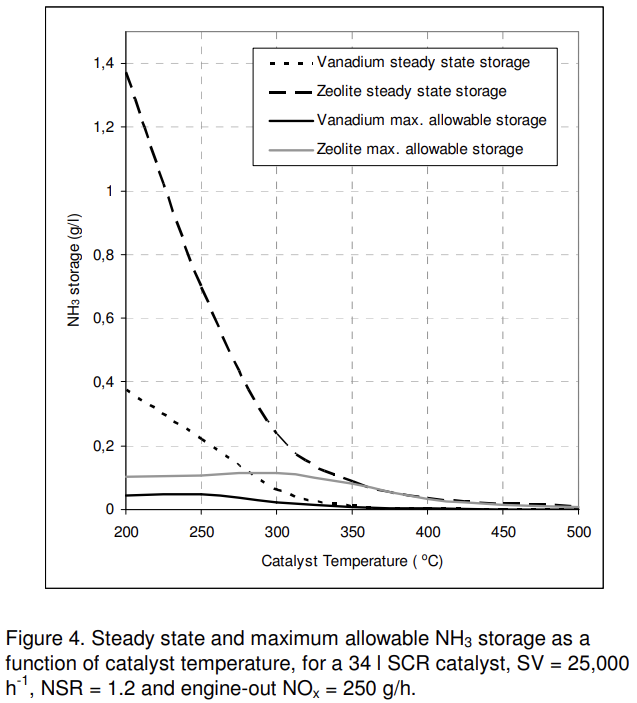
\includegraphics[width = 0.8\textwidth]{./figs/storage_capacity/sae.png}
            \caption*{Results from \cite{willems2007closed}}
        \end{figure}
    \end{minipage}
    \begin{minipage}{0.49\textwidth}
        \begin{figure}[H]
            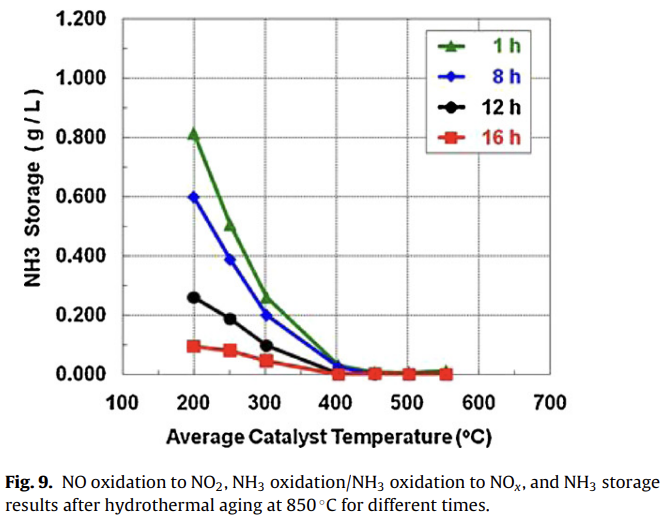
\includegraphics[width = \textwidth]{./figs/storage_capacity/th1.png}
            \caption*{Results from \cite{schmieg2012thermal}}
        \end{figure}
    \end{minipage}
    \begin{minipage}{0.49\textwidth}
        \begin{figure}[H]
            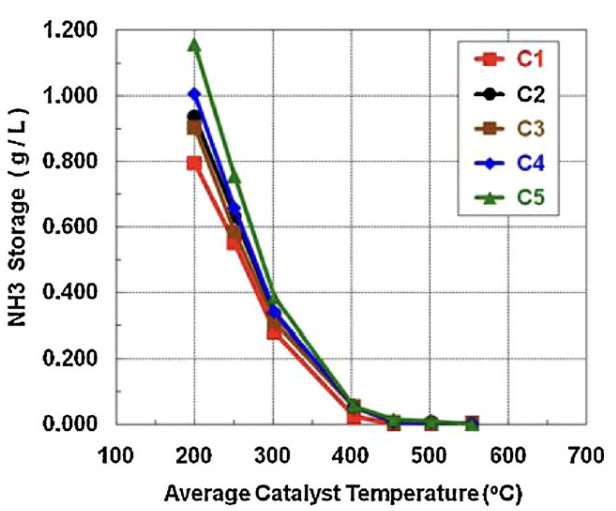
\includegraphics[width = \textwidth]{./figs/storage_capacity/th_2.png}
            \caption*{Results from \cite{schmieg2012thermal}}
        \end{figure}
    \end{minipage}
    \begin{minipage}{0.49\textwidth}
        \begin{figure}[H]
            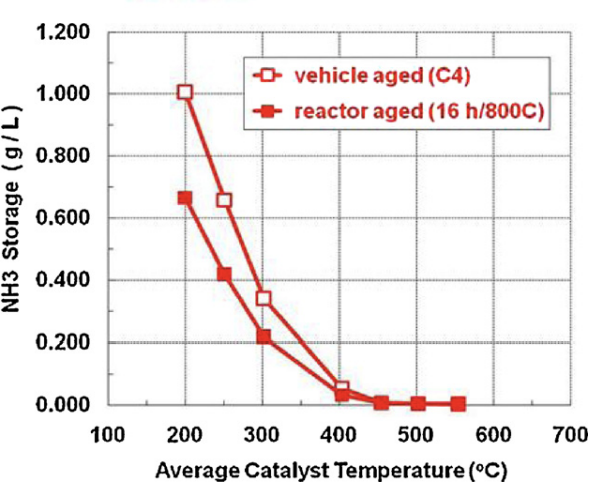
\includegraphics[width = \textwidth]{./figs/storage_capacity/th_3.png}
            \caption*{Results from \cite{schmieg2012thermal}}
        \end{figure}
    \end{minipage}
    \caption{Temperature effects of catalyst storage capacity}
\end{figure}


\subsection{Catalyst aging factor}

\itbf{Assumption}: The aged catalyst results in small changes in
$S_1, S_2$.

The above assumption is valid if the catalyst's operating range is limited to a
small range of storage capacity.

Using small perturbation,
\begin{align*}
    \delta \Theta &= \lr{\frac{\delta S_1}{S_1} - \delta S_2T} S_1 e^{-S_2 T}\\
    \implies \Theta_{aged} &= \Theta + \delta \Theta = \lr{1 + \frac{\delta S_1}{S_1} - \delta S_2T} S_1 e^{-S_2 T}
\end{align*}

Let,
\begin{align*}
    a(T) &= 1 + \frac{\delta S_1}{S_1} - \delta S_2T = a_1 + a_2 T
\end{align*}

Thus, $a$ is the factor by which the storage capacity is reduced due to the
catalyst's aging. Hence, for optimal performance:
\begin{align*}
    a > a_{min} \quad \forall T \in [T_{min}, T_{max}]
\end{align*}

\itbf{Note}: The above definition is consistent with that of the literature
\cite{ma2017observer}. The major difference lies in its derivation and
assumptions. Also, \cite{ma2017observer} considers aging factor as temperature
independent fraction and has no minimum value for classifying the catalyst as aged.

Consequently, \itbf{the catalyst aging detection problem becomes estimating the
aging factor and testing if it is bellow $a_{min}$ in presence of
uncertainties}.


\subsubsection{Aging factor estimation problem formulation}
Given the simplified non-linear concentration dynamics for SCR-ASC
reactions with internal dynamics and sensor corss-sensitivity
\ref{eqn::ctrl_state}. Estimate the total molar
Ammonia storage capacity of the catalyst [$\Theta(t, T)$]. Then,
\begin{align*}
    a(t, T) &= \frac{\Theta(t, T)}{\Theta(0, T)} = a_1 + a_2 T
\end{align*}


\itbf{No fault condition:}
$$ a(t, T) > a_{min} \quad \forall T \in [T_{min}, T_{max}], \: t > 0$$

\bigskip

We have the following high-level steps in fault-diagnosis:
\begin{enumerate}
    \item Estimate cross-sensitivity factor $\chi$.
    \item Estimate the lumped model parameters $f_{\bullet}, g_{\bullet}$.
    \item Using $f_{\bullet}, g_{\bullet}$, estimate $\Theta(t, T)$.
\item Estimate $a(t, T)$ and propagate all the uncertainties down to
$\delta_{a}$, the uncertainty in $\hat a$.
    \item Check for no-fault condition:
\begin{align*}
    \hat a(t, T) \pm \delta_a > a_{min} \quad \forall T \in [T_{min}, T_{max}]
\end{align*}
\end{enumerate}

